\documentclass{standalone}
\usepackage{tikz}
\usepackage{circuitikz}
\usetikzlibrary{positioning}

\begin{document}
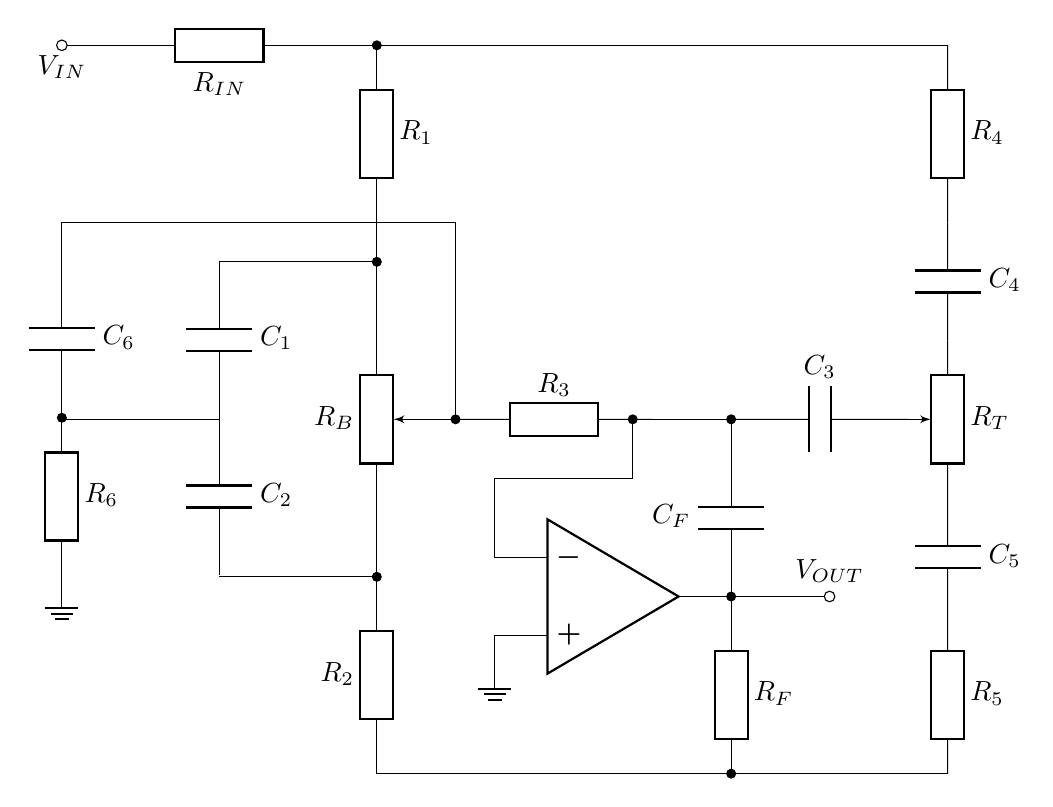
\begin{tikzpicture}
	\draw (5.5, 11.25) to[european resistor, l=$R_{IN}$] (1.5, 11.25);
	\draw (5.5, 9) to[european resistor, l_=$R_1$] (5.5, 11.25);
	\draw (5.5, 4.5) to[european resistor, l_=$R_2$] (5.5, 2);
	\draw (9, 6.5) to[european resistor, l_=$R_3$] (6.5, 6.5);
	\draw (12.75, 11.25) to[european resistor, l=$R_4$] (12.75, 9);
	\draw (12.75, 4) to[european resistor, l=$R_5$] (12.75, 2);
	\draw (1.5, 4.52) to[european resistor, l_=$R_6$] (1.5, 6.52);
	\draw (10, 4) to[european resistor, l=$R_F$] (10, 2);

	\draw (5.5, 8.5) to[european potentiometer, l_=$R_B$] (5.5, 4.5);
	\draw (12.75, 5.5) to[european potentiometer, l_=$R_T$] (12.75, 7.5);

	\draw (3.5, 8.5) to[capacitor, l=$C_1$] (3.5, 6.52);
	\draw (3.5, 6.52) to[capacitor, l=$C_2$] (3.5, 4.52);
	\draw (10, 6.5) to[capacitor, l=$C_3$] (12.25, 6.5);
	\draw (12.75, 9) to[capacitor, l=$C_4$] (12.75, 7.5);
	\draw (12.75, 5.5) to[capacitor, l=$C_5$] (12.75, 4);
	\draw (1.5, 8.52) to[capacitor, l=$C_6$] (1.5, 6.52);
	\draw (10, 6.5) to[capacitor, l_=$C_F$] (10, 4);

	\node[op amp] at (8.5, 4.25) {};

	\draw (1.5, 6.5) -| (3.5, 6.52);
	\draw (1.5, 8.52) -| (1.5, 9) -- (6.5, 9) -- (6.5, 6.5);
	\draw (3.5, 4.5) -- (5.5, 4.5);
	\draw (5.5, 8.5) -- (5.5, 9);
	\draw (3.5, 8.5) -- (5.5, 8.5);
	\draw (5.5, 11.25) -- (12.75, 11.25);
	\draw (5.5, 2) -| (12.75, 2);
	\draw (6.06, 6.5) -- (6.5, 6.5);
	\draw (7.31, 3.76) |- (7, 3.76) -- (7, 3.5);
	\draw (7.31, 4.74) -| (7, 4.75) -- (7, 5.75) -- (8.75, 5.75) -- (8.75, 6.5);
	\draw (9, 6.5) -- (10, 6.5);
	\draw (9.69, 4.25) |- (11.25, 4.25);

	\node[ground] at (1.5, 4.52) {};
	\node[ground] at (7, 3.5) {};
	\node[circ] at (1.5, 6.52) {};
	\node[circ] at (10, 2) {};
	\node[circ] at (10, 4.25) {};
	\node[circ] at (10, 6.5) {};
	\node[circ] at (5.5, 8.5) {};
	\node[circ] at (5.5, 4.5) {};
	\node[circ] at (5.5, 11.25) {};
	\node[circ] at (6.5, 6.5) {};
	\node[circ] at (8.75, 6.5) {};
	\node[ocirc, scale=1.2] at (1.5, 11.25) {};
	\node[ocirc, scale=1.2] at (11.25, 4.25) {};

	\node[below=0cm of {1.5, 11.25}] {$V_{IN}$};
	\node[above=0.05cm of {11.25, 4.25}] {$V_{OUT}$};

\end{tikzpicture}
\end{document}